\subsection{Анализ опасных и вредных производственных факторов на рабочем месте}
Производственный фактор, воздействие которого на работающего человека, в определённых условиях приводит к травме или другому внезапному резкому ухудшению здоровья, называется опасным. Если же производственный фактор приводит к заболеванию или снижению работоспособности, то его считают вредным (ГОСТ 12.0.002-80)~\cite{OT9}.

В зависимости от уровня и продолжительности воздействия вредный производственный фактор может стать опасным.

В целях предупреждения травматизма и профессиональных заболеваний при воздействии опасных и вредных производственных факторов (ОПФ и ВПФ) на предприятиях применяются меры по их предупреждению и устранению, а также снижению степени воздействия на работников.

Согласно ГОСТ 12.0.003 – 74 ``Опасные и вредные производственные факторы. Классификация''~\cite{OT8}, все опасные и вредные производственные факторы делятся по природе воздействия на следующие группы:

\begin{enumerate}
\item физические;
\item химические;
\item биологические;
\item психофизиологические.
\end{enumerate}
Из всех перечисленных факторов в наших условиях работы на организм действуют только физические и психофизиологические опасные и вредные производственные факторы.

К физическим опасным и вредным производственным факторам можно отнести:

\begin{enumerate}
\item недостаточная освещённость помещения. Качество поступающей информации во многом зависит от освещения. Недостаточное освещение не только утомляет глаза, но и вызывает утомление организма в целом. При неудовлетворительном освещении снижается производительность труда и увеличивается брак;
\item повышенное значение напряжения в электрической цепи, замыкание которой может произойти через тело человека. Системный блок и монитор ЭВМ питаются от бытовой сети переменного тока напряжением 220 В частотой 50 Гц;
\item повышенный уровень неионизирующих \ электромагнитных полей и излучений в рабочей зоне;
\item повышенный уровень шума. Одним из важнейших параметров, наносящим ущерб для здоровья и снижающим производительность труда, является шум. Шум может создаваться как работающим оборудованием, установками кондиционирования воздуха, работающими осветительными приборами дневного света, так и проникать извне. Действие шума различно: он затрудняет разборчивость речи, вызывает снижение работоспособности, повышает утомляемость, вызывает необратимые изменения в органах слуха человека. Шум воздействует не только на органы слуха, но и на весь организм человека через центральную нервную систему. Ослабляется внимание, ухудшается память, снижается реакция, увеличивается число ошибок при работе;
\item неудовлетворительное состояние параметров микроклимата. Количество теплоты, выделяемое человеком в окружающую среду, и охлаждающая способность среды должны быть адекватны, то есть человек должен себя чувствовать комфортно. В противном случае у человека возникают беспокоящие его температурные ощущения холода или перегрева, отрицательно сказывающиеся на его самочувствии и работоспособности;
\item возможность возникновения пожара. Во время работы с электрооборудованием в сети переменного тока может возникнуть перегрев и воспламенение самого оборудования или его обшивки.
\end{enumerate}
К психофизиологическим факторам согласно ГОСТ 12.0.003-74~\cite{OT8} можно отнести такие факторы как:

\begin{enumerate}
\item физические (статические) перегрузки;
\item нервно-психические перегрузки.
\end{enumerate}
В процессе работы инженер не подвержен воздействию химических и биологических производственных факторов.

\subsection{Требования и защитные мероприятия в области БЖД}
\subsubsection{Освещение}
Информация, которую человек получает из внешнего мира, поступает в основном через зрительный канал. Поэтому качество информации, получаемой посредством зрения, во многом зависит от освещения. Неудовлетворительное освещение может исказить информацию; кроме того, оно утомляет не только зрение, но вызывает утомление организма в целом. Неправильное освещение может также, являться причиной травматизма: плохо освещённые опасные зоны, слепящие лампы и блики от них, резкие тени ухудшают или вызывают полную потерю ориентации работающих.

На практике пользуются двумя видами освещения — естественным и искусственным.

При освещении помещений, согласно СНиП 23-05-95 ``Естественное и искусственное освещение''~\cite{OT6}, необходимо соблюдать следующие требования:

\begin{enumerate}
\item естественное освещение должно осуществляться через светопроёмы, ориентированные преимущественно на север и северо-восток, и обеспечивать коэффициент естественной освещённости не ниже 1.2 \%;
\item освещенность рабочего места пользователя ПЭВМ должно быть 200-400 лк (IV (в) разряд зрительных работ, ``Естественное и искусственное освещение СНиП 23-05-95''~\cite{OT6});
\item для освещения зоны расположения документов допускается установка светильников местного освещения. Местное освещение не должно создавать бликов на поверхности экрана и увеличивать освещённость экрана более 300 лк;
\item в поле зрения оператора должно отсутствовать прямая и отражённая блескость;
\item на рабочем месте оператора должно быть ограничена пульсация освещённости от газоразрядных источников света;
\item в качестве источников света при искусственном освещении должны применяться преимущественно люминесцентные лампы типа ЛБ. Допускается применение ламп накаливания в светильниках местного освещения.
\end{enumerate}
Рассчитаем реальную освещённость на рабочем месте. Целью данного расчёта является проверка соответствия освещённости в рабочем помещении норме освещённости согласно СНиП 23-05-95~\cite{OT6}.

Проведём проверочный расчёт освещённости методом коэффициента использования светового потока.

Освещённость определяется по формуле:
\begin{equation}
\label{eq:sunny}
E=\frac{F{\cdot}N{\cdot}\eta }{k{\cdot}S{\cdot}z},
\end{equation}

где \textit{F} – световой поток каждой из ламп, лм;

\textit{N} – число источников света;

\textit{$\eta $} – коэффициент использования светового потока;

\textit{k} – коэффициент запаса, учитывающий запыление светильников и износ источников света;

\textit{S} – площадь помещения, м\textsuperscript{2};

\textit{z} – коэффициент неравномерности освещения.

Определим данные для расчёта.

Коэффициент \textit{k} для помещений, освещаемых лампами и при условии чистки светильников не реже двух раз в год берётся равным 1,4 – 1,5.

При оптимальном расположении светильников коэффициент неравномерности \textit{z} равен 1,1 – 1,2.

Коэффициент использования светового потока $\eta$ зависит от типа светильника, коэффициента отражения светового потока от стен $\textit{Р}_{\textit{С}}$, потолка $\textit{Р}_{\textit{П}}$, пола $\textit{Р}_{\textit{ПОЛА}}$, а также геометрических размеров помещения и высоты подвеса светильников, что учитывается одной комплексной характеристикой – индексом помещения:

\begin{equation}
\label{eq:index_opt_flor}
I=\frac S{h{\cdot}(A+B)},
\end{equation}

где \textit{h} – высота подвеса светильников над рабочей поверхностью, м;

\textit{А} – ширина помещения, м;

\textit{В} – длина помещения, м.

Рассматриваемое помещение имеет следующие характеристики:

\begin{itemize}
\item ширина \foreignlanguage{english}{\textit{A}} – \foreignlanguage{english}{5} м;
\item длина \foreignlanguage{english}{\textit{B}}\foreignlanguage{english}{ }– 7 м;
\item площадь помещения \foreignlanguage{english}{\textit{S}}\foreignlanguage{english}{ }– 35 м\textsuperscript{2};
\item высота до осветительного прибора \foreignlanguage{english}{\textit{h}} – 3 м;
\item количество ламп \foreignlanguage{english}{\textit{N}} – 8;
\item поправочный коэффициент \foreignlanguage{english}{\textit{Z}} – 1.1;
\item световой поток одной лампы \foreignlanguage{english}{\textit{F}} – 1340 лм;
\item коэффициент запаса \foreignlanguage{english}{\textit{k}} – 0.4.
\end{itemize}
Тогда индекс помещения по формуле (\ref{eq:index_opt_flor}):
%$$ I = \dfrac{S}{h\cdot(A+B)} = \dfrac{35}{3\cdot\(5+7\)} = 0.97$$
Используя этот коэффициент по светотехнической таблице, находим, что для нашего помещения коэффициент \textit{$\eta $ }равен 53 \%.

Теперь можно произвести расчёт освещённости по формуле (\ref{eq:sunny}):

$$
E=\dfrac{F\cdot N \cdot \eta}{k \cdot S \cdot z} = \dfrac{1340{\cdot}8{\cdot}0.53}{35{\cdot}1.1{\cdot}0.4}=369,
$$
Согласно СНиП 23-05-95, освещённость рассматриваемого помещения находится в диапазоне оптимального освещения, т.к. по нормативам для разряда зрительной работы \foreignlanguage{english}{IV} (\textit{в}) норма освещённости находится в диапазоне от 200 лк до 400 лк. Это означает, что мощность и количество осветительных приборов для данного помещения выбраны правильно, и не требуется дополнительного освещения.
\subsubsection{Микроклимат}

Выбор типа \textit{производственного помещения} определяется технологическим процессом, возможностью борьбы с шумом, вибрациями и загрязнением воздуха. Наличие больших оконных проёмов и фонарей должно обеспечивать хорошую естественную освещённость. В помещении обязательно устройство вентиляции.

Объем и площадь производственного помещения, которые должны проходиться на каждого работающего по санитарным нормам, должны быть не менее 20 $m^{3}$ и 6 $m^{2}$ соответственно. Высота производственных помещений не должна быть менее 4 м. Стены и потолки необходимо сооружать из малотеплопроводных материалов, не задерживающих осаждение пыли. Полы должны быть тёплыми, эластичными, ровными и нескользкими.

Под оптимальными микроклиматическими условиями понимают такие сочетания параметров микроклимата, которые при детальном и систематическом воздействии на человека обеспечивают сохранение нормального функционального и теплового состояния организма.

На организм человека и работу вычислительной техники большое влияние оказывает относительная влажность воздуха. При влажности воздуха до 40\% становится хрупкой основа магнитной ленты, повышается износ магнитных головок, выходит из строя изоляция проводов, также возникает статическое электричество при движении носителей информации в ЭВМ. При относительной влажности воздуха более 75-80\% снижается сопротивление изоляции, изменяются рабочие характеристики ЭВМ, возрастает интенсивность их отказов.

Скорость движения воздуха тоже оказывает влияние на функциональную деятельность человека, так как способствует испарению влаги с кожного покрова. А это, в свою очередь, приводит либо к высыханию кожи, либо к нарушению теплового равновесия организма, т.е. скорость движения воздуха, может иметь положительное значение с точки зрения физического охлаждения лишь до температуры воздуха $35-36^{\circ} C$. При дальнейшем повышении температуры окружающей среды единственным путём теплопередачи является испарение. Однако при повышении температуры свыше $40^{\circ} C$ движение даже относительно сухого воздуха может оказываться неблагоприятным фактором. Горячий воздух отдаёт теплоту телу, и подвижность воздуха в этом случае приводит не к охлаждению, а, наоборот, к нагреванию.

В машинном зале рекомендуется поддерживать температуру и влажность воздуха постоянными. Атмосферное давление должно быть в допустимых пределах, так как при пониженном, например, давлении ухудшается отвод тепла от элементов ЭВМ, снижаются изоляционные свойства узлов и устройств ЭВМ.

Воздух должен в значительной степени очищаться от пыли. ЭВМ, имеющие в своём составе устройства ввода-вывода на магнитных дисках, требуют этого, так как пылинки, попадающие на рабочую поверхность диска, могут привести к повреждению магнитной головки или поверхности диска. Пыль, оседающая на устройства и узлы ЭВМ, ухудшает теплоотдачу, может образовывать токопроводящие цепи, вызывает износ подвижных частей, нарушает контакты и приводит к засорению лёгких у работающего персонала.

Не менее важно и значение освещения. При неудовлетворительном освещении зрительная способность снижается, и могут появиться заболевания глаз. Правильно выполненная система освещения имеет большое значение в снижении травматизма, уменьшая потенциальную опасность многих производственных факторов; создаёт нормальные условия для работы органов зрения и повышает общую работоспособность организма.

С целью создания нормальных условий работы установлены нормы производственного микроклимата (ГОСТ 12.1.005-88)\cite{OT10}. Эти нормы устанавливают оптимальные и допустимые значения температуры, относительной влажности и скорости движения воздуха для рабочей зоны помещений, оборудованных компьютерами с учётом тяжести выполняемой работы и сезона года.

\begin{table}[!ht]
\caption{Оптимальные и допустимые нормы температуры, относительной влажности и скорости движения воздуха в рабочей зоне производственного помещения}
\centering
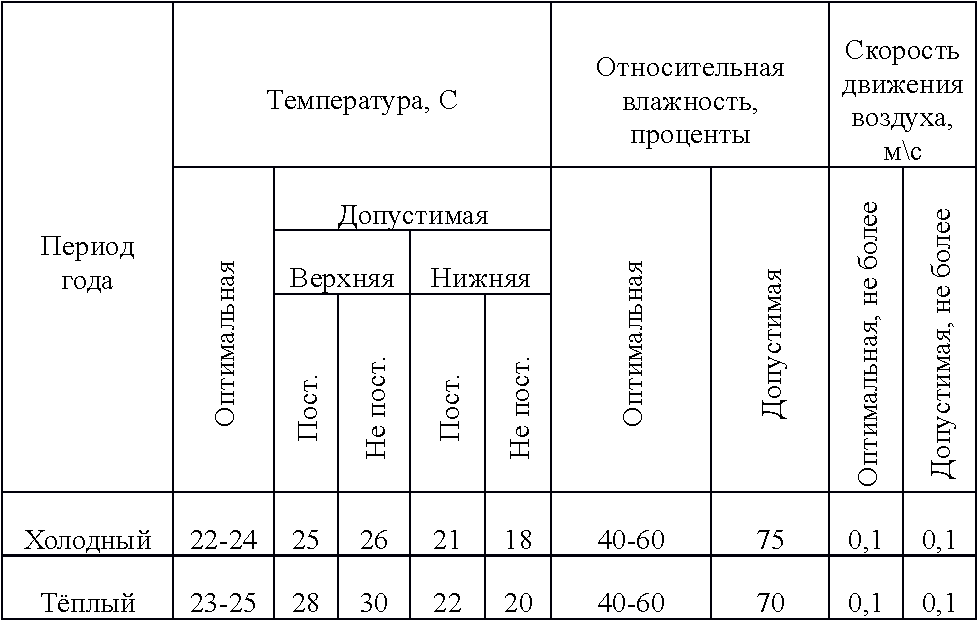
\includegraphics[page=1, width=1\linewidth]{secure_table.pdf}
\label{tab:micro_climat}
\end{table}

\subsubsection{Электробезопасность}

Электрические установки, к которым относится ЭВМ и стенд, представляют для человека потенциальную опасность. В процессе эксплуатации или при проведении профилактических работ человек может соприкасаться с частями, находящимися под током. Согласно классификации помещений по электробезопасности (ПУЭ – 7-е издание) рабочий кабинет относится к помещениям без повышенной опасности, характеризующимся наличием следующих условий:

\begin{enumerate}
\item напряжение питающей сети, 220 В;
\item напряжение питающей сети, 380 В;
\item относительная влажность воздуха, не более $75\%$;
\item средняя температура не более $25^{\circ}C$.
\end{enumerate}
При нормальном режиме работы опасность поражения электрическим током невелика, однако, возможны режимы, называемые аварийными, когда происходит случайное электрическое соединение частей оборудования, находящихся под напряжением с заземлением конструкциями. Опасность поражения электрическим током существует всюду, где используются электроустановки, поэтому помещения без повышенной опасности нельзя назвать безопасными.

Любое из воздействий тока (термическое, электролитическое, механическое и биологическое) может привести к электрической травме, т. е. к повреждению организма, вызванному действием электрического тока или электрической дуги.

Основными техническими способами и средствами защиты от поражения током, согласно ГОСТ Р 12.1.009-2009 ``Система стандартов безопасности труда. Электробезопасность''~\cite{OT11}. Общие требования и номенклатура видов защиты'', являются: защитное зануление, выравнивание потенциалов, защитное заземление, электрическое разделение сети, изоляция токоведущих частей, оградительные устройства и другое.

Согласно ``Система стандартов безопасности труда. Электробезопасность. Предельно допустимые значения напряжений прикосновения и токов'' ЭВМ и стенд, на которых производится работа, относятся к классу электробезопасности 01 (имеет рабочую изоляцию, элемент для заземления и провод без заземляющей шины для подключения питания).

Напряжения прикосновения и токи, протекающие через тело человека при нормальном (неаварийном) режиме электроустановки не должны превышать значений, указанных в таблице \ref{tab:voltage_amper}

\begin{table}[!ht]
\caption{Таблица предельно допустимых значений напряжений прикосновения и токов}
\centering
\includegraphics[page=2, width=1\linewidth]{secure_table.pdf}
\label{tab:voltage_amper}
\end{table}

Для исключения возможности поражения электрическим током проведены следующие меры:

\begin{enumerate}
\item токоведущие части, находящиеся под напряжением, изолированы;
\item корпуса приборов заземлены;
\item заземляющие проводники видны, а места их соединений скреплены резьбовыми соединениями.
\end{enumerate}
\subsubsection{Пожарная безопасность}

Для выполнения требований по пожарной безопасности (ГОСТ 12.1.004-91 ССБТ. Пожарная безопасность)\cite{OT4} необходимо удаление оборудования друг от друга на расстояние не менее 60-80 см.

Опорные части из изоляционных материалов, удерживающие детали, предназначенные для подключения к сети, а также изолирующие корпуса должны быть изготовлены из материалов, не представляющих опасность при возникновении коротких замыканий внутри блока или при нагреве, вызываемого плохим контактом внешних проводов.

Необходимо также наличие пожарного инвентаря и проведение инструктажей.

Приведём возможные причины возникновения пожаров:
\begin{enumerate}
\item наличие твёрдых горючих веществ;
\item опасная перегрузка сетей, которая ведет за собой сильный разогрев токопроводящих проводников и загорания изоляции;
\item короткие замыкания;
\item пуск оборудования после ремонта.
\end{enumerate}
Для предупреждения пожаров от коротких замыканий, перегрузок необходим правильный выбор монтаж и соблюдение установленного режима эксплуатации электрических сетей, дисплеев и других устройств.

\subsubsection{Электромагнитные неионизирующие излучения}

Длительное воздействие электромагнитных полей промышленной частоты (50 Гц) приводит к расстройствам в головном мозге и центральной нервной системе. В электрическом поле (ЭП) атомы и молекулы поляризуются.
Полярные молекулы ориентируются по направлению распространения электромагнитного поля, что изменяет ориентацию клеток или цепей молекул, ослабляя биохимическую активность белковых молекул.
В результате у человека наблюдаются головная боль в височной и затылочной областях, вялость, ухудшение памяти, боли в области сердца, угнетённое настроение, апатия, своеобразная депрессия с повышенной чувствительностью к яркому свету и интенсивному звуку, расстройство сна, сердечно-сосудистой системы (ССС), органов пищеварения, дыхания, повышенная раздражительность.
Могут наблюдаться функциональные нарушения в ЦНС, а также изменения в составе крови.

Воздействие постоянного магнитного поля (ПМП) и с частотой 50 Гц на человека проявляется в индуцировании в теле человека вихревых токов.

При длительном систематическом воздействии могут возникнуть изменения функционального состояния нервной системы, иммунной системы и сердечно-сосудистой системы. Длительное воздействие ЭМП промышленной частоты может спровоцировать онкологические заболевания.

Предельно допустимые значения напряжённости электрического и магнитного полей промышленной частоты в зависимости от времени их воздействия устанавливаются СанПиН 2.2.4.1191-03 ``Электромагнитные поля в производственных условиях''\cite{OT12}. Согласно этому нормативному документу пребывание в ЭП промышленной частоты напряжённостью до 5 кВ/м допускается в течение всего рабочего дня.

При работе на персональном компьютере расстояние от монитора до глаз пользователя должно быть не менее 50 см. Исследования показали, что с уменьшением расстояния на каждые 10 см уровень электромагнитного излучения возрастает в среднем в 1,5 раза, а с увеличением расстояния с 50 до 60 см уменьшение уровня электромагнитного поля идёт в той же зависимости.

\begin{table}[!ht]
\caption{Допустимые значения параметров неионизирующих электромагнитных излучений}
\centering
\includegraphics[page=3, width=1\linewidth]{secure_table.pdf}
\label{tab:min_neoinige_elwave}
\end{table}

\subsubsection{Допустимые уровни звукового давления и звукового шума}

Шум на исследовательском рабочем месте создаётся вентиляционной системой ПЭВМ и печатающим устройством. В процессе рабочего дня принтер включается по мере необходимости, поэтому шум следует квалифицировать как непостоянный, прерывистый.

Основными физическими величинами, характеризующими шум, являются интенсивность, звуковое давление и частота. Согласно ГОСТ 12.1.003-83 ``Система стандартов безопасности труда. Шум''\cite{gost_sec_noize}. Общие требования безопасности'' для оценки шума используют частотный спектр измеряемого уровня звукового давления, выраженного в дБ, в октавных полосах частот, который сравнивают с предельным спектром, приведены в таблице \ref{tab:arm_noise_locate}.

\begin{table}[!ht]
\caption{Значения предельно допустимых уровней шума на рабочих местах производительных предприятий}
\centering
\includegraphics[page=4, width=1\linewidth]{secure_table.pdf}
\label{tab:arm_noise_locate}
\end{table}

(1) – помещение технологических бюро, лаборатории для теоретических работ;

(2) – помещения управлений, рабочие комнаты;

(3) – кабины наблюдения и дистанционного управления с речевой телефонной связью, помещение и участки тонкой сборки;

(4) – лаборатории для проведения экспериментальных работ;

(5) – постоянные рабочие места и рабочие зоны в производственных помещениях и на территории предприятий.

Уровень шумов от компьютеров и вентиляторов в помещении соответствует пункту (1) таблицы 7.2.3. Согласно~\cite{gost_sec_ergo_33} шум, создаваемый вентиляторами и компьютерами, постоянный и не превышает установленного звукового давления.

\subsection{Требования эргономики и технической эстетики}
Для создания благоприятных условий труда в лаборатории необходимо учитывать психофизические особенности человека, а также общую гигиеническую обстановку. Большое значение в создании оптимальных условий труда имеют складывающиеся в трудовом коллективе взаимоотношения между студентами, которые принято называть социальным климатом. Человек, находящийся в состоянии нервного возбуждения допускает много ошибок при работе с технологической документацией.

С эстетической точки зрения помещение и оборудование должны быть окрашены в спокойные тона (синие, голубые, зелёные) успокаивающие и уменьшающие зрительное утомление. Окраска стен и дверей помещения должна иметь мягкие переходы без резких яркостных контрастов. В рабочем помещении стены покрашены бежевой краской, потолок покрыт белой плиткой, двери окрашены в синий цвет. Это даёт хорошее отражение и рассеяние света.

Важную роль играет планирование рабочего места, которое должно удовлетворять требованиям удобства выполнения работ и экономии энергии, времени инженера, удобства обслуживания устройств ЭВМ и соблюдения правил охраны труда. Рабочее место должно обеспечивать удобство выполнения работы в помещении сидя, стоя и соответствовать требованиям ГОСТ 12.2.032-78\cite{gost_sec_ergonom_32} и ГОСТ 12.2.033-78~\cite{gost_sec_ergo_33}. Необходим учёт эргономических свойств человека, подбор вспомогательных предметов оборудования (столы, и т. п.), удобных для использования на рабочем месте. Для этого требуется рациональная расстановка оборудования, оптимальная организация рабочего места (правильный выбор основного технологического оборудования, удобство выполнения работ). Рабочее место при выполнении действий в положении сидя должно соответствовать нормам~\cite{gost_sec_ergonom_32}s.

Определим требования к рабочему месту: обеспечение возможности удобного выполнения работ, учёт физической тяжести труда, учёт размеров рабочей зоны, учёт технологических особенностей процесса выполнения работ. Параметры рабочего места инженера приведены в таблице \ref{tab:arm_ing_locate}.

\begin{table}[!ht]
\caption{Параметры рабочего места инженера}
\centering
\includegraphics[page=5, width=1\linewidth]{secure_table.pdf}
\label{tab:arm_ing_locate}
\end{table}

В рабочей зоне необходимо исключение резких и подвижных теней, отблесков. При планировке рабочего места необходимо учитывать зоны досягаемости рук оператора при расположении дисплея, клавиатуры, органов управления системы и периферийных устройств. Эти зоны, установленные на основании антропометрических данных человеческого тела, дают возможность рационально разместить как по горизонтали, так и по вертикали все элементы рабочего места.

Правильная организация рабочего места оператора ЭВМ предусматривает также соблюдение следующих параметров:

\begin{enumerate}
\item высота мыши с клавиатурой (62-88) см (над уровнем пола);
\item высота экрана (над уровнем пола) (90-128) см;
\item расстояние от экрана до края стола (0-115) см;
\item наклон экрана от минус $15\textsuperscript{0}$ до плюс $20\textsuperscript{0}$ к нормальному его положению;
\item расстояние от глаз оператора до экрана должно быть в пределах от 40 до 80 см.
\end{enumerate}
В состав рабочего места входят учебный стенд, персональный компьютер, видеомонитор, клавиатура.

Органы управления, к которым относятся клавиатура и манипулятор ``мышь'' ЭВМ \ \ расположены в зоне досягаемости, ограниченной длиной руки, т.е. от 70 до 80 см. Такое расположение обеспечивает равномерную нагрузку обеих рук оператора.

К системам отображения информации, на данном рабочем месте, относятся: видеомонитор ЭВМ. Видеомонитор распложён в зоне пространства отображения информации ($\pm15^{\circ}C$ от нормальной линии взгляда), что обеспечивает оптимальный зрительный поиск.

В результате анализа можно сделать вывод, что организация рабочего места, на котором выполнялась дипломная работа, удовлетворяет перечисленным выше требованиям правильной организации рабочего места оператора ЭВМ. Так, как и остальные условия работы в помещении являются удовлетворительными (микроклимат, освещение и т.д.), о чем писалось выше, то согласно ГОСТ 12.2.032-78.ССБТ\cite{gost_sec_ergonom_32} данное рабочее место работника можно считать соответствующим общим эргономическим требованиям.

\subsection{Общие требования безопасности перед началом, вовремя, по окончании работы и в случае аварийных ситуаций}
\subsubsection{Требования безопасности перед началом работы}

Перед началом работы работник должен:

\begin{itemize}
\item проверить на рабочем месте наличие и пригодность средств защиты, инструмента и приспособлений, а также наличие электрического фонаря, средств пожаротушения, плакатов или знаков безопасности;
\item проверить достаточность освещения рабочей зоны и на обслуживаемом оборудовании (отсутствие перегоревших ламп) наличие плафонов на светильниках;
\item ознакомиться с работами производимыми предыдущими работниками, прочитав об этом в ``Оперативном журнале'';
\item при обнаружении, каких-либо отклонений в работе САР доложить технику.
\end{itemize}
\subsubsection{Требования безопасности во время работы}
\begin{itemize}
\item использовать инструмент и приспособления, предназначенные только для выполнения данной работы. Не допускать применения случайных приспособлений и предметов вместо инструмента;
\item следует выполнять только ту работу, которая поручена;
\item импульсные трубопроводы, на которых производится ремонт оборудования КИПиА, необходимо перекрыть при помощи запорной арматуры и снять давление;
\end{itemize}
Запрещается во время работы:

\begin{itemize}
\item эксплуатировать неисправное оборудование, а также оборудование с неисправными или отключёнными устройствами аварийного отключения блокировок, защит и сигнализации;
\item применять для отмывки и обезжиривания деталей и оборудования керосин, бензин, бензол, ацетон и другие, горючие и легковоспламеняющиеся вещества, при уборке помещений и оборудования горючие вещества, а также хлорпроизводные углеводороды;
\end{itemize}
\begin{itemize}
\item при обнаружении дефектов на оборудовании немедленно сообщить об этом своему руководству и руководству обслуживаемого объекта;
\item во время работы необходимо поддерживать чистоту и порядок на рабочем месте;
\item во время работы соблюдать противопожарные правила, знать местонахождение первичного противопожарного инвентаря, уметь его применять и не допускать использование противопожарных средств не по назначению;
\end{itemize}
\subsubsection{Действия в аварийных ситуациях}

При возникновении аварии или ситуации, которые могут привести к нежелательным последствиям, необходимо прекратить работу, принять меры по предупреждению несчастных случаев, выхода из строя оборудования, сообщить технику или заведующему кафедры, в котором возникла аварийная ситуация, а также принять меры обеспечения безопасности других лиц;

При возникновении аварийных ситуаций необходимо:

\begin{itemize}
\item прекратить работу;
\item обесточить оборудование, если это угрожает жизни и здоровью персонала;
\item принять меры по предупреждению несчастных случаев, выхода из строя оборудования;
\item сообщить руководству;
\end{itemize}

\begin{itemize}
\item при возникновении пожара необходимо немедленно вызвать пожарную охрану, отключить электрооборудование, находящееся в зоне пожара. Приступить к тушению пожара с помощью первичных средств пожаротушения. Для тушения пожара в электроустановках необходимо применять только углекислотные и порошковые огнетушители.
\end{itemize}
\subsubsection{Требования безопасности по окончании работы}

По окончании работы работник должен:

\begin{itemize}
\item выключить оборудование;
\item привести в порядок рабочее место.
\end{itemize}